%%%%%%%%%%%%%%%%%%%%%%%%%%%%%%%%%%%%%%%%%%%%%%%%%%%%%%%%%%%%%%%%%
%        Contents: Bachelorarbeit, HS Fulda        %
%                          06.09.2022                        %
%---------------------------------------------------------%
%                            Konzept.tex                     %
%                        by Carina Möller                   %
%                    cary_moeller@gmx.de              %
%%%%%%%%%%%%%%%%%%%%%%%%%%%%%%%%%%%%%%%%%%%%%%%%%%%%%%%%%%%%%%%%%

\chapter[Konzept der Transformationsengine]{Konzept der Transformationsengine} \label{KO}

Das Ziel dieser Bachelorarbeit ist es, eine Transformationsengine zu bauen, die bestimmte Daten von verschiedenen Produkten in eine vorgegebene Excel"=Vorlage schreibt. Nach einer allgemeinen Vorstellung der Problemstellung und der Rahmenbedingungen, werden die Konzepte zu drei möglichen Lösungsansätzen näher erläutert. Die letzten beiden werden später in Kapitel\nbs\ref{IM} implementiert. 

\section{Allgemeines} \label{AL}
\begin{figure}[b]
 \centering
 \censorbox{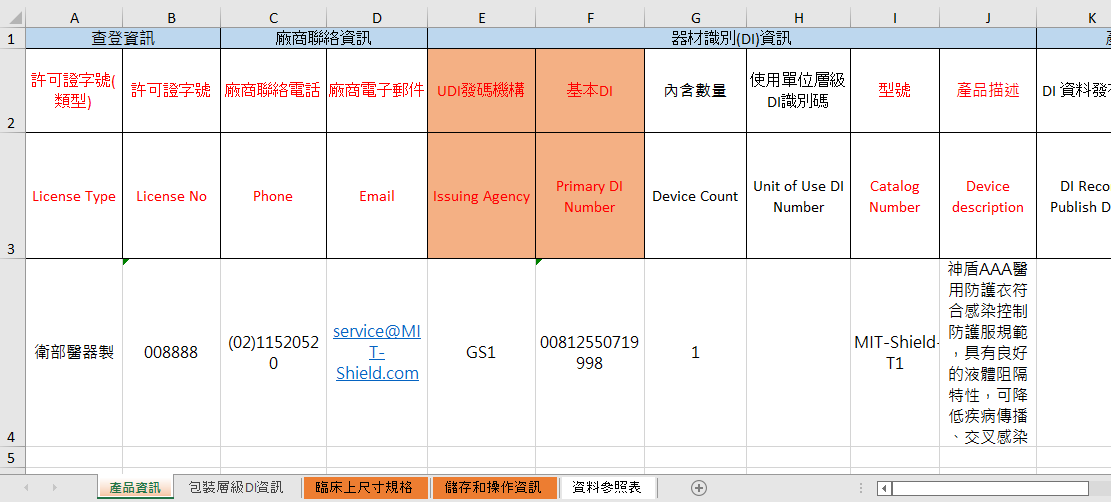
\includegraphics[width=0.95\textwidth]{Bilder/Taiwan1}}
 \caption[Excel-Vorlage für Taiwan -- Ausschnitt 1]{Ausschnitt 1 der Excel-Vorlage von Taiwan}
 \label{fig:t1} 
\end{figure}

Die Transformationsengine soll ausgewählte Produktdaten aus der \xblackout{UDI Platform} von \xblackout{p36} in Excel"=Arbeitsmappen schreiben. Form, Struktur und Inhalt der Excel"=Dateien ist dabei behördlich vorgegeben. Die erfolgreich ausgefüllten Dateien werden später bei den Behörden hochgeladen, um die Produkte samt zugehöriger Informationen in deren Datenbanken zu registrieren\nbs --\nbs dies findet allerdings außerhalb der Transformationsengine statt.

Die verschiedenen Behörden publizieren jeweils ihre individuelle Excel"=Vorlage, die zum Import verwendet werden muss. Wie bereits in Kapitel\nbs\ref{UDI} erläutert, führen in den nächsten Jahren verschiedene Gesundheitsministerien ein UDI"=System ein, bei dem man die Produkte per Excel"=Datei registrieren muss. Als Erstes stand die SFDA aus Saudi"=Arabien auf der Agenda von \xblackout{p36}, bis sie die Veröffentlichung des Excel"=Templates kurzfristig um ein Jahr verschoben haben. Dies ist leider gängige Praxis seitens der Behörden, sodass es umso wichtiger ist, dass die Plattform flexibel ist. Für Ende des Jahres ist nun die Einbindung von Taiwan geplant\nbs --\nbs hier existiert bereits eine Vorlage inklusive Übersetzung. Drei Auszüge mit einem eingetragenen Beispielprodukt sind in den Abbildungen\nbs\ref{fig:t1},\nbs\ref{fig:t2} und\nbs\ref{fig:t3} zu sehen.

\begin{figure}[htbp]
 \centering
 \censorbox{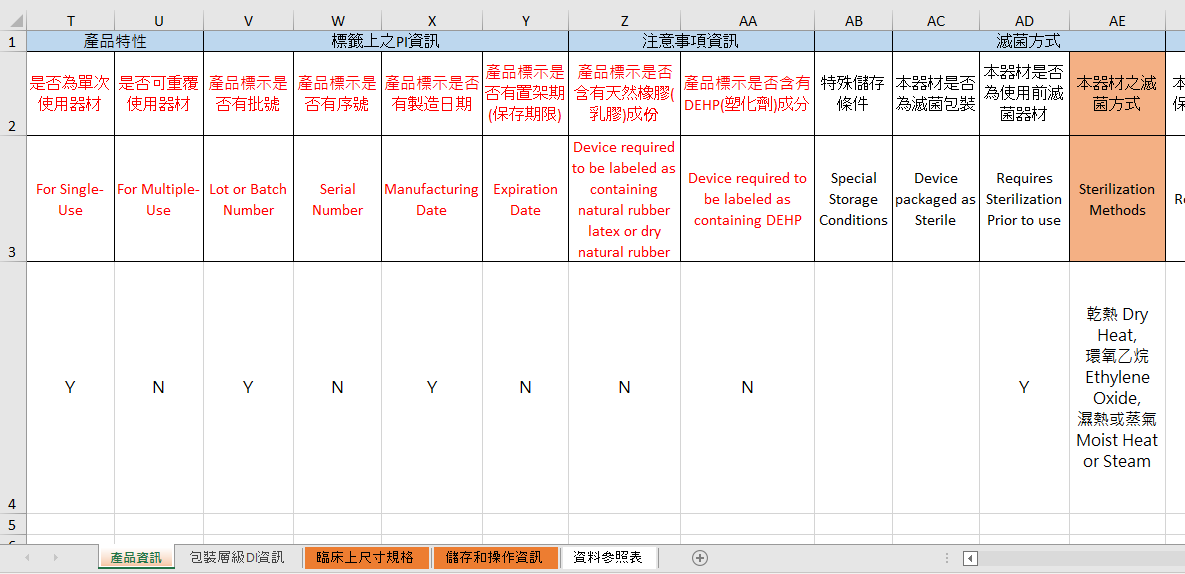
\includegraphics[width=0.95\textwidth]{Bilder/Taiwan2}}
 \caption[Excel-Vorlage für Taiwan -- Ausschnitt 2]{Ausschnitt 2 der Excel-Vorlage von Taiwan}
 \label{fig:t2}
\end{figure}
\begin{figure}[htbp]
 \centering
 \censorbox{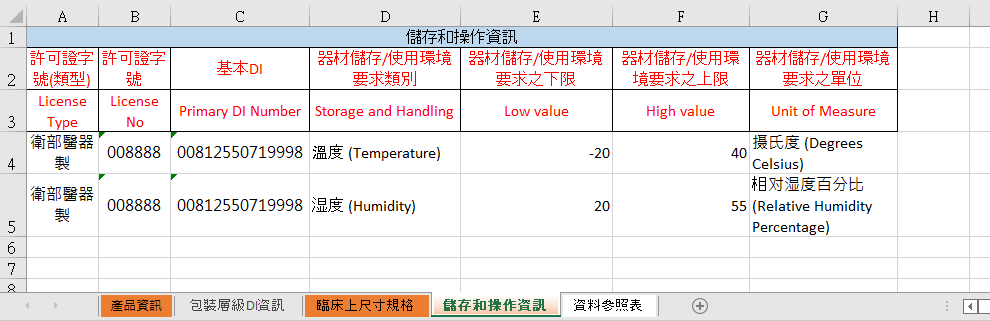
\includegraphics[width=0.95\textwidth]{Bilder/Taiwan3}}
 \caption[Excel-Vorlage für Taiwan -- Ausschnitt 3]{Ausschnitt 3 der Excel-Vorlage von Taiwan}
 \label{fig:t3}
\end{figure}

Die geforderten Datenelemente sind dabei vielschichtig\nbs --\nbs von der UDI und deren Vergabestelle, über Informationen zu Hersteller, Modell, Material und Inhaltsstoffe bis hin zur Produktion, Lagerung oder Sterilisationsmethoden sowie viele weitere Details. Einige Beispiele sind in Abbildung\nbs\ref{fig:de} aufgelistet.
Momentan unterschneidet \xblackout{p36} insgesamt fast 200 verschiedene Datenelemente für fünf Behörden (EU, FDA, NMPA, MFDS und SFDA). Diese sind in den Agency"=Device"=Models (ADM) implementiert, zusätzlich gibt es das übergeordnete Common"=Device"=Model (CDM), welches die gängigsten Elemente einer hypothetischen "`typischen"' Behörde in sich vereint. Unter den Datenelementen befinden sich auch 15 sogenannte komplexe Elemente, die wiederum aus einfachen Elementen bestehen. Mit jeder zusätzlichen Behörde ergeben sich in der Regel neue Elemente, außerdem können Kunden Anpassungen und Erweiterungen initiieren (die allerdings für die Weiterleitung an die Behörde nicht maßgeblich sind bzw. sein dürfen). Die Daten sind intern im JSON"=Format gespeichert. 

\begin{figure}[htbp]
 \centering
 \censorbox{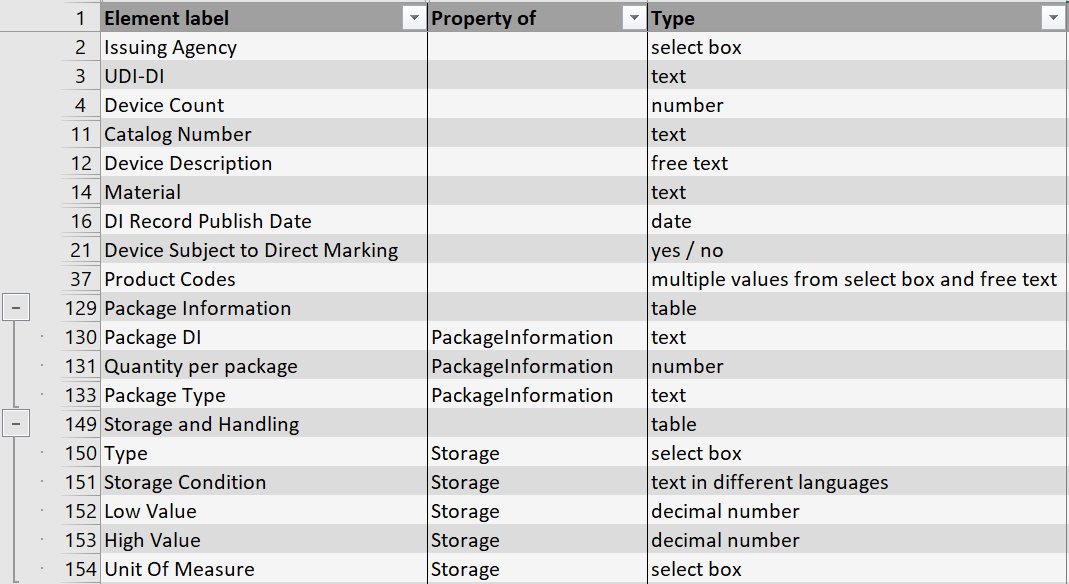
\includegraphics[width=0.8\textwidth]{Bilder/dataelements}}
 \caption[Beispiele für Datenelemente]{verschiedene Datenelemente}
 \label{fig:de}
\end{figure}

Es gibt viele fundamentale Produktinformationen, die von allen Behörden gefordert werden, aber auch einige Unterschiede besonders bei spezielleren Daten. Die am häufigsten verwendeten Elemente hat \xblackout{p36} im CDM zusammengefasst. \\
Zusätzlich können die Datentypen oder -formate variieren, wenn eine Behörde bestimmte Werte für ein Datenelement erwartet oder bei lokalen Datums"~/""Zeitangaben. Dies umfasst ebenfalls die Kodierung von Wahrheitswerten: Während manche Behörden direkt mit \texttt{true} und \texttt{false} als Boolean arbeiten, akzeptieren andere zum Beispiel nur \texttt{Y} bzw. \texttt{N} als valide Eingabe, so wie es in Taiwan der Fall ist (siehe Abbildung\nbs\ref{fig:t2}). Des Weiteren kann sich die Wertemenge individueller Datenelemente unterscheiden, denn verschiedene Behörden kodieren bestimmte Eigenschaften mit anderen Wertelisten. Dazu müssen zunächst die \xblackout{p36}"=internen Werte in die behördenspezifische Sprache "`übersetzt"' werden.

Neben den einfachen Datenelementen mit 1\,:\,1"=Beziehung, die in einer einzigen Zelle abgebildet werden können, gibt es auch die bereits erwähnten komplexen Datenelemente mit 1\,:\,$n$"=Beziehung. Diese werden in zusätzlichen Arbeitsblättern über ggf. mehrere Zeilen angegeben, wie z.\,B. anhand der beiden Lagerungswerte in Abbildung\nbs\ref{fig:t3} zu erkennen ist. Hier hat ein Produkt zwei Einträge beim komplexen Element "`Storage and Handling"'\nbs --\nbs es sind Informationen zur Temperatur sowie zur Luftfeuchtigkeit hinterlegt. Der Schlüssel für die einzelnen Arbeitsblätter ergibt sich in der Regel aus der eindeutigen UDI-DI (hier mit "`Primary DI Number"' bezeichnet, vgl. Kapitel\nbs\ref{UDI}); als zusätzliche Informationen werden in diesem Fall noch Lizenztyp und -nummer wiederholt. Darüber hinaus sind auch exotischere Einträge möglich, wie z.\,B. eine Liste von Sterilisationsmethoden in Spalte AE von Abbildung\nbs\ref{fig:t2}. Hier wird das komplexe Element "`Sterilisation"' zu einem Eintrag in einer Zeile verschmolzen.\\
Rot eingefärbte Spaltennamen sind obligatorisch, schwarz beschriftete Spalten optional. Welche Elemente verpflichtend sind, variiert von Behörde zu Behörde.

Die meisten großen Medizinprodukte"=Hersteller haben nicht nur einige wenige Produkte am Markt platziert, sondern bieten vornehmlich eine breite Produktpalette an, die sich zusätzlich durch eine Vielzahl unterschiedlicher Ausprägungen und Variationen weiter auffächert\nbs --\nbs und das in den verschiedensten Verpackungseinheiten. Multipliziert man die Farben, Formen und Größen, entsteht eine enorme Menge an Devices, die alle ihre eigene UDI besitzen und im System registriert werden müssen. Hierzu empfiehlt sich der Massen"=Upload. Die Transformationsengine muss in der Lage sein, viele Produkte (in der Größenordnung von 1.000--10.000) simultan in die Excel"=Vorlage zu schreiben.

Zusammengefasst ergeben sich unter anderem die folgenden Anforderungen:
\begin{table}[htbp]
\centering
%\setlength\extrarowheight{2pt} headline ist hübsch, aber alle zeilen sind dadurch breiter
\begin{tabular}{ |M{1cm}|p{8.5cm}| }
\hline
Nr. & funktionale Anforderungen\TBstrut\\
\hhline{==}
\anf{trans} & Transformation von Produktdaten in Excel-Vorlage\Tstrut\\
\anf{bool} & Mapping von Wahrheitswerten\\
\anf{date} & Mapping von Datums- und Zeitformaten\\
\anf{elem} & Mapping von Wertelisten einzelner Datenelemente\Bstrut\\
\hline
\end{tabular}

\vspace*{0.3cm}

\begin{tabular}{ |M{1cm}|p{8.5cm}| }
\hline
Nr. & nichtfunktionale Anforderungen\TBstrut\\
\hhline{==}
\anf{gen} & generisch bzgl. verschiedener Behörden\Tstrut\\
\anf{bf} & benutzerfreundliche Wartung bei Änderungen\\
\anf{mu} & Massen-Upload möglich, in annehmbarer Zeit\Bstrut\\
\hline
\end{tabular}
\caption{\label{tab:fnfa}Funktionale und nichtfunktionale Anforderungen}
\end{table}







\section{Spezifischer Ansatz} \label{HC}

Die naheliegendste und simpelste Lösung ist es sicherlich, für jede Behörde spezifisch und individuell die Transformation hart zu kodieren.\\
Hierbei könnte für jede Behörde eine eigene Klasse entstehen, in der exklusiv das Format der Excel"=Arbeitsmappe sowie deren individueller Inhalt spezifiziert wird. Diese Abbildung kann einfach starr aufgeschrieben werden. \\
Aus Zeitgründen wurde dieser Ansatz allerdings weder tiefergehend verfolgt noch implementiert, sondern er sei hier nur in der Theorie erwähnt, als Vergleichsgrundlage für die spätere Evaluierung. 

Stattdessen liegt der Fokus dieser Bachelorarbeit auf den folgenden beiden generischen Ansätzen, deren Implementierung unabhängig von den Behörden funktioniert. 




\section{Generischer Ansatz mit Excel-Datei} \label{ED}

Da \xblackout{p36} die Transformationsengine nicht nur für eine Behörde nutzen möchte, sondern grundsätzlich mit einer langfristigen und entsprechend generischen Denkweise agiert, müssen die behördenspezifischen Informationen extern abgespeichert werden anstatt im Quellcode enthalten sein. Die Behördenanforderungen beschreiben quasi eine Abbildung von den Spalten der Excel"=Mappe auf bestimmte Datenelemente. Inhalt der Abbildung ist dann das Produktportfolio, das man sich als ein $n$"=dimensionales Tupel einzelner Produkte vorstellen kann, welches auf $n$ Zeilen abgebildet wird (bei 1\,:\,1"=Beziehungen).

Die erste Idee bestand darin, die Definition dieser Abbildung in die Excel"=Arbeitsblätter auszulagern.\\
Konkret wird das mit \bib{JMESPath}"=Ausdrücken (siehe Kapitel\nbs\ref{JQL}) in der Excel"=Vorlage umgesetzt. Das heißt die \xblackout{Solution Manager} müssen zunächst in der Vorbereitung das Excel"=Template der Behörde entsprechend ausfüllen und auf der \xblackout{Plattform} hinterlegen. Dies geschieht einmalig, wenn die Behörde neu ins System aufgenommen wird bzw. immer dann, wenn Änderungen auf Seiten der Behörde oder \xblackout{p36} auftreten. Hierfür muss in jede Spalte, die mit Daten zu füllen ist, in der Zeile, in die das erste Produkt geschrieben werden soll, stattdessen der \bib{JMESPath}"=Ausdruck eingegeben werden, und zwar innerhalb spitzer Klammern. 
Falls die Spalte verpflichtend ausgefüllt werden muss, wird dies mit einem einleitenden Ausrufezeichen \texttt{!} gekennzeichnet\nbs --\nbs der Syntax ist also \texttt{<!JMESPath"=Ausdruck>}. Die Notation wurde willkürlich festgelegt und kann angepasst werden. Abbildung\nbs\ref{fig:jms1} gibt einen kleinen Einblick, wie eine solche Excel"=Datei aussehen könnte. Die Wahl von \bib{JMESPath} als Abfragesprache ist dabei weitestgehend arbiträr und sie könnte auch durch eine vergleichbare Sprache ersetzt werden.

\begin{figure}[htbp]
 \centering
 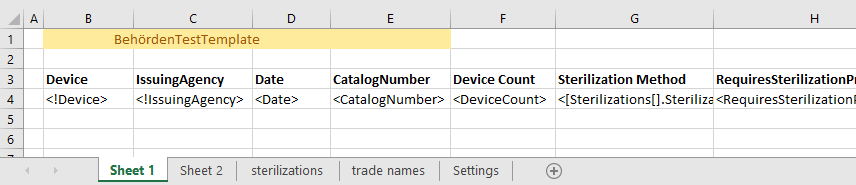
\includegraphics[width=0.75\textwidth]{Bilder/JMESPath1}
 \caption[\bib{JMESPath}-Ausdrücke in der Excel-Vorlage einer Behörde]{\bib{JMESPath}-Ausdrücke in der Excel-Vorlage einer Behörde}
 \label{fig:jms1}
\end{figure}
Diese Ausdrücke können beliebig kompliziert werden. Die ersten Spalten in Abbildung\nbs\ref{fig:jms1} beinhalten lediglich die Bezeichnungen der Datenelemente und sind in vielen Fällen ausreichend. Durch einen Punkt gelangt man eine Ebene tiefer, außerdem ist Filtern per Fragezeichen möglich, vgl. Abschnitt\nbs\ref{JM}. Mit\\
\centerline{\texttt{<TradeNames[?TradeNameLanguage == 'EN'].TradeName>}}
wird beispielsweise nur der englische Handelsname in die Zelle geschrieben.\\
Darüber hinaus gibt es noch einige Spezialfälle. \bib{JMESPath} stellt verschiedene eingebaute Funktionen zur Verfügung, die man per Pipe"=Symbol \texttt{|} hintereinander ausführen kann, um so weitergehende Selektionen bzw. Manipulationen durchzuführen. Auf zwei Beispiele wird im Folgenden eingegangen.
\begin{itemize}
\item Das Datenelement \texttt{ProductionIdentifier} fasst bei \xblackout{p36} verschiedene Kennwörter in einem Array zusammen. In der Excel"=Datei hat allerdings jedes Kennwort seine eigene Spalte\nbs --\nbs ist der Identifikator im Array enthalten, wird dies bei der Behörde mit \texttt{true} angezeigt und entsprechend bei Absenz mit \texttt{false}. Das gewünschte Ergebnis erzielt der Ausdruck\\
\centerline{\texttt{<ProductionIdentifier | contains(@,'IDENTIFIER')>} ,\phantom{mmmm}}\\
wobei \texttt{IDENTIFIER} durch das jeweilige Schlüsselwort ersetzt werden muss. 
\item Die bereits erwähnten Sterilisationsmethoden sollen alle zusammen in einer Zelle aufgelistet werden, jeweils mit Kommas getrennt. Dies lässt sich durch\\
\phantom{mmmm}\texttt{<[Sterilizations[].SterilizationMethod, }\\
\phantom{mmmm<[}\texttt{Sterilizations[].OtherSterilizationMethods] | }\\
\phantom{mmmm<}\texttt{[].to\_string(@) | join(', ',@)>}\\
realisieren. Hier werden zunächst alle Datenfelder, die Sterilisationsmethoden beinhalten, in einem Array gesammelt, danach in Strings umgewandelt und zuletzt vereinigt. Das \texttt{@} dient als Platzhalter für das jeweils aktuelle Element im Array. Die Umwandlung in Strings ist nötig, weil die Funktion \texttt{join} nur für String"=Arrays definiert ist.
\end{itemize}

\subsection{Zusätzliche Einstellungen} \label{zM}

Um ergänzende Informationen zu übertragen, wie beispielsweise die behördenspezifische Darstellung von Wahrheitswerten, wird ein zusätzliches Arbeitsblatt namens "`Settings"' in die Vorlage eingefügt. Ein Beispiel zeigt Abbildung\nbs\ref{fig:jms2}. Die Projektion der beiden Wahrheitswerte muss unter dem Schlüsselwort "`Boolean"' angegeben werden. Weitere Mappings für einzelne Datenelemente sind unter der Elementbezeichnung in spitzen Klammern möglich. Die Bezeichnung muss mit dem Ausdruck übereinstimmen, der in der Spalte angegeben wurde, in der das Datenelement verwendet wird. Hier bietet sich eine Excel"=interne Verlinkung an, anstatt einen längeren Ausdruck erneut abzutippen oder zu kopieren. Es muss jeweils der Wert in der \xblackout{p36}"=internen Schreibweise eingegeben werden und in der Zelle rechts daneben der Ziel"=Wert in Behördensprache. Dies ist in Zeile 11 bzw. 20 in Abbildung\nbs\ref{fig:jms2} zu sehen, bei der z.\,B. mit Zahlen kodierte Sterilisationsmethoden in ihre chinesische Bezeichnung überführt werden.

\begin{figure}[htb]
 \centering
 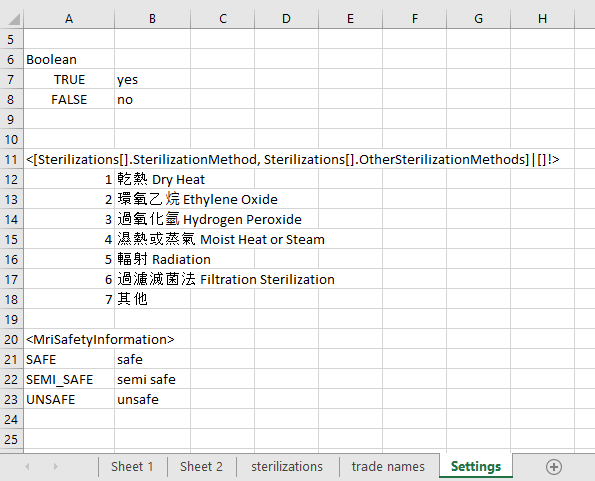
\includegraphics[width=0.75\textwidth]{Bilder/JMESPath2}
 \caption[Das Settings-Arbeitsblatt aus Ansatz\nbs\ref{ED}]{Das Settings-Arbeitsblatt}
 \label{fig:jms2}
\end{figure}
Beim Einlesen der Vorlage werden die Informationen im Settings"=Sheet verarbeitet, in Hashtabellen abgespeichert und das Arbeitsblatt anschließend gelöscht, sodass es letztendlich nicht bei der Behörde mit hochgeladen wird. Entscheidend beim Einlesen ist die vertikale Anordnung der Elemente bzw. ihrer Werte und dass eine Liste von Werte"=Paaren jeweils mit einer Leerzeile abgeschlossen wird.
Es besteht die Möglichkeit über dieses Arbeitsblatt noch weitere Informationen oder andere besondere Einstellungen einfließen zu lassen, deren Logik allerdings erst in der Transformationsengine implementiert werden muss. 

Zusammengefasst besteht das Konzept also darin, dass die Metainformationen zur Abbildung zwischen Excel"=Datei und Produktdaten einmalig zu Beginn in die Excel"=Vorlage geschrieben werden, wenn die Behörde in die \xblackout{UDI Platform} aufgenommen wird. Dies kann noch durch ein zusätzliches Arbeitsblatt mit besonderen "`Settings"' individualisiert werden. 
Bei regulatorischen Änderungen muss entsprechend die Excel"=Vorlage bearbeitet werden, in der Regel bleibt aber der Code der Transformationsengine unberührt und dient für alle Behörden gleichermaßen.




\section{Generischer Ansatz mit Mapping-Datei} \label{MD}

Eine Variation vom bisherigen Ansatz\nbs\ref{ED} ist es, die Abbildung von den Spalten der Excel"=Datei zu den Produktdaten in einer zusätzlichen Datei zu speichern. Sie wird im Folgenden Mapping"=Datei genannt. Dadurch bleibt die Excel"=Vorlage der Behörde unberührt und die Informationen übersichtlicher. 

Zunächst wurde als Mapping eine normale Textdatei mit selbst gestalteter Notation anhand von Keywörtern und rudimentärem Parsing gewählt, bei dem der eingelesene Text nach den Schlüsselwörtern abgesucht wird. Dies ist aber unnötig umständlich, sodass in einem zweiten Schritt auf eine YAML"=Datei umgestellt wurde. Die Auszeichnungssprache YAML wurde 2001 von Clark Evens entworfen und ist in\nbs\cite{yaml} spezifiziert. Das YAML"=Format ist sehr gut für Menschen lesbar sowie leicht zum Editieren. Im Gegensatz zu JSON oder XML ist es noch reduzierter durch die Absenz von Klammern und Anführungszeichen und damit noch übersichtlicher\nbs --\nbs der Vergleich wird in\nbs\cite{json:yaml} vertieft.

Im Unterschied zu Ansatz\nbs\ref{ED}, welcher mit \bib{JMESPath} arbeitet, wird hier die JSON"=Abfragesprache \bib{JSONata} (siehe Abschnitt\nbs\ref{Jata}) verwendet. Beide Sprachen eignen sich in beiden Ansätzen und sind theoretisch austauschbar, aber um beide auszutesten und weil \bib{JSONata} noch umfangreicher ist, wurde gewechselt. Die Vor"~ und Nachteile werden später in Kapitel\nbs\ref{EV} detaillierter erläutert. 

Die Mapping"=Datei ist strukturell in zwei Teile untergliedert.\\
Ein Teil beschreibt die Arbeitsblätter: Er wird mit dem Schlüssel \texttt{SheetMappings} eingeleitet und enthält eine assoziative Liste von einzelnen Arbeitsblättern, die wiederum aus Schlüssel"=Werte"=Paaren bestehen. Als Key dient dabei der Name des Arbeitsblattes in der Excel"=Datei. Hierbei werden unter anderem auch chinesische Schriftzeichen unterstützt, was insbesondere für Taiwan ein wichtiger Punkt ist. Einige Sonderzeichen werden von Excel selbst ausgeschlossen, ebenso zu lange Namen, die mehr als 31 Zeichen enthalten. 
Zur Visualisierung ist in Quelltext\nbs\ref{code:md1} ein Auszug einer beispielhaften Mapping"=Datei dargestellt.
\begin{lstlisting}[language=yaml,caption={Beispiel einer Mapping-Datei für \texttt{SheetMappings}},label=code:md1]
SheetMappings:
  Sheet 1:
    row: 4
    columns: 
      B: Device
      C: Date
(*\label{line:ml3}*)      D: >
        *B*$exists(DeviceCount) ? DeviceCount : "NA"
      E: $join(Sterilizations.SterilizationMethod.$string(),", ")
(*\label{line:ml5}*)      F: >-
        *B*RequiresSterilizationPriorUse ? 1 : 0
      G: CatalogNumber
      H: TradeNames[TradeNameLanguage = "EN"].TradeName
      I: $contains($join(ProductionIdentifier),"BATCH_NUMBER")
(*\label{line:ml4}*)      J: |
        *B*"RUBBER" in ProductionIdentifier
      K: '"DEHP" in ProductionIdentifier'
      M: MriSafetyInformation
      N: UnitOfUseDi
      L: PackageInformation
(*\label{line:mc1}*)    mandatoryColumns: [B, G, D] 
      
  (*\rmfamily 產品資訊*):
    row: 2
    category: TradeNames
    columns: 
      A: Device 
      B: IssuingAgency
(*\label{line:ml1}*)      C: *B*'TradeNames.($exists(TradeNameLanguage)?TradeNameLanguage:null)'
(*\label{line:ml2}*)      D: *B*"TradeNames.($exists(TradeName) ? TradeName : null)"
(*\label{line:mc2}*)    mandatoryColumns: 
    - *B*A 
    - *B*B
\end{lstlisting}
Für jedes Arbeitsblatt müssen die folgenden Informationen angegeben werden:
\begin{itemize}
\item Unter \texttt{row} wird die Start"=Zeile gespeichert, ab der die Produktdaten eingetragen werden können.
\item Dem Schlüssel \texttt{columns} ist ein Mapping aller zu füllenden Spalten zugeordnet. Hierbei dienen die Excel"=Spaltennamen jeweils als Key und als Value wird der \bib{JSONata}"=Ausdruck angegeben, über welchen später die gewünschte Produktinformation gefiltert wird.
\item In \texttt{mandatoryColumns} kann eine Liste verpflichtender Spalten übergeben werden. Dies kann kompakt in eckigen Klammern wie in Zeile\nbs\ref{line:mc1} erfolgen oder über mehrere Zeilen mit Bindestrichen wie ab Zeile\nbs\ref{line:mc2}.
\item Mit \texttt{category} kann das komplexe Datenelement angeben werden, dessen Inhalte in das jeweilige Arbeitsblatt geschrieben werden sollen. Ist die Kategorie gesetzt, werden nur für die Produkte Zeilen erzeugt, die tatsächlich auch Einträge unter besagtem komplexen Datenelement haben. 
\end{itemize}
Dabei spielt weder die Groß"~ und Kleinschreibung der Spaltennamen eine Rolle, noch in welcher Reihenfolge die Wertepaare eingegeben werden. Zur Übersicht bietet sich eine alphabetische Anordnung allerdings an. \\
Die \bib{JSONata}"=Ausdrücke können beliebig komplex werden und mehrere Zeilen umfassen oder Zeichen enthalten, die man in YAML escapen muss, wie beispielsweise Doppelpunkte (\texttt{:}), Doppelkreuze (\texttt{\#}) oder Anführungsstriche zu Beginn (\texttt{``} bzw. \texttt{`}). Dafür bietet YAML mehrere Möglichkeiten: Der gesamte Ausdruck kann in Anführungszeichen gesetzt werden (siehe Zeile\nbs\ref{line:ml1} und\nbs\ref{line:ml2}), oder man leitet einen ggf. mehrzeiligen Ausdruck mit den Symbolen \texttt{>} bzw. \texttt{|} ein. Dies ist in den Zeilen\nbs\ref{line:ml3} und\nbs\ref{line:ml4} dargestellt. Mit dem Größer"=Als"=Zeichen \texttt{>} werden alle internen Zeichenumbrüche gelöscht, wohingegen der Pipe"=Befehl \texttt{|} die einzelnen Zeilen erhält. Mit einem optionalen Bindestrich \texttt{-} dahinter wie in Zeile\nbs\ref{line:ml5} wird auch kein Zeilenumbruch am Ende des Blocks hinzugefügt. So lassen sich beliebig lange Funktionen in \bib{JSONata} schreiben. 

Der andere Teil der Mapping"=Datei beschreibt die Abbildungen für einzelne Datenelemente oder besondere Formate. Er wird mit dem Schlüsselwort \texttt{ElementMappings} eingeleitet. Hier ist als Beispiel ein Auszug abgebildet:
\begin{lstlisting}[language=yaml,caption={Beispiel einer Mapping-Datei für \texttt{ElementMappings}}]
ElementMappings:
 Boolean:
   true: Y
   false: N
   
 Date:
(*\label{line:date}*)   yyyy-MM-dd: yyyy\/m\/d
   d.MM.yyyy: m/d/yy
   
 SterilizationMethod:
   (*1\color{red}: \color{black}\rmfamily{乾熱}*) *B*Dry Heat
   (*2\color{red}: \color{black}\rmfamily{環氧乙烷}*) *B*Ethylene Oxide
   (*3\color{red}: \color{black}\rmfamily{過氧化氫}*) *B*Hydrogen Peroxide
   (*4\color{red}: \color{black}\rmfamily{濕熱或蒸}*) *B*Moist Heat or Steam
   (*5\color{red}: \color{black}\rmfamily{過濾滅菌法}*) *B*Filtration Sterilization
   
 MriSafetyInformation:
   SAFE: 0
   NOT_SAFE: 1
   SEMI_SAFE: 2
\end{lstlisting}
%Das hat kompett gesponnen bei chinesischen zeichen, daher musste ich die escapen und dann die farbe switchen und und ... 
Unter dem Stichwort \texttt{Boolean} können behördenspezifische Wahrheitswerte gesetzt werden, wie zum Beispiel \texttt{Y} und \texttt{N} wie in Abbildung\nbs\ref{fig:t2}. Außerdem ist es via \texttt{Date} möglich, Datums"~ und Zeitangaben passend für die Excel"=Vorlage zu formatieren. Dabei muss als Schlüssel das interne Format in \xblackout{p36} angegeben werden und als Wert das gewünschte Excel"=Format. Mit \texttt{m/d/yy} zeigt Excel das Datum automatisch in der lokalen Standard"=Schreibweise an. Für speziellere Formate ist gegebenenfalls das Escapen der Schrägstriche notwendig, wie in Zeile\nbs\ref{line:date}. Genau wie im vorherigen Ansatz können zusätzlich Mappings für einzelne Datenelemente spezifiziert werden. Diese müssen hier lediglich mit dem Namen des Elements eingeleitet werden, nicht dem gesamten \bib{JSONata}"=Ausdruck analog zu Abschnitt\nbs\ref{zM}. Durch die YAML"=Notation können einfache Zuweisungen von \xblackout{p36}"=internen Werten zu den behördenspezifischen Übersetzungen intuitiv angegeben werden. Dabei werden alle primitiven Datentypen sowie Strings unterstützt, auch in gemischter Form.

\subsection{JSON-Schema}\label{JSch}
Da die Mapping"=Datei eine ganz bestimmte Struktur einhalten muss, wird diese anhand eines Schemas überprüft. YAML ist zwar eine Obermenge von JSON und hat Funktionalitäten, die über JSON hinausgehen, aber für die meisten YAML"=Dateien eignet sich dennoch ein JSON"=Schema zur Validierung ihrer Form. So auch bei der Transformationsengine. In\nbs\cite{json:schema} und\nbs\cite[S.\,21--29]{json:wallace} wird aus der praktischen Sicht heraus vertieft, wie ein JSON"=Schema aufgebaut ist und welche Möglichkeiten es gibt, die Struktur einer JSON"=Datei zu beschreiben, während Pezoa\,et.\,al. in\nbs\cite{json:schema:def} das JSON"=Schema theoretisch beleuchten und formal definieren.

Das Schema selbst wird ebenfalls im JSON"=Format geschrieben, in diesem Fall entsprechend Version\nbs v6 der JSON"=Schema"=Spezifikation. Sie wird zu Beginn mit dem Schlüsselwort \texttt{\$schema} angegeben. Das gesamte Schema ist im Quelltext\nbs\ref{code:schema} im Anhang\nbs\ref{AJS} zu finden. Es besteht aus den beiden JSON"=Objekten \texttt{SheetMappings} und \texttt{ElementMappings}, wobei letzteres auch weggelassen werden darf, falls keinerlei extra Mappings nötig sind.  \\
In \texttt{SheetMappings} können unter \texttt{additionalProperties} die Namen der Arbeitsblätter als Objekt hinzugefügt werden, welche die Eigenschaften \texttt{row} und \texttt{columns} verpflichtend haben müssen, während \texttt{category} und die Liste der \texttt{mandatoryColumns} optional sind. Bei der Startzeile muss es sich entsprechend der Excel"=Konvention um einen Integer beginnend ab Eins handeln. Außerdem muss mindestens eine Spalte angegeben werden. Die Spaltennamen werden ebenso durch Excel vorgegeben und müssen aus ein bis zwei Buchstaben bestehen. Dieses Muster muss auch im Array \texttt{mandatoryColumns} eingehalten werden. Auf die Beachtung von Groß"~ und Kleinschreibung kann verzichtet werden, da intern ohnehin alles in Großbuchstaben umgewandelt wird. \\
Das Objekt \texttt{ElementMappings} kann die Eigenschaften \texttt{Boolean} (welches wiederum nur das Mapping für \texttt{true} und \texttt{false} beinhalten darf) und \texttt{Date} besitzen, sowie zusätzliche Objekte für Abbildungen einzelner Datenelemente. Hierbei sind Kombinationen aus allen möglichen einfachen Typen von Zahlen über Wahrheitswerte bis hin zu Strings erlaubt.

Durch das Schema können falsche Eingaben, die später zu Fehlern führen, bereits zu Beginn identifiziert werden. Ursprünglich war die Transformationsengine so konzipiert, dass alle durch die Schemavalidierung erkannten, fehlerhaften Pfade des JsonNodes \texttt{mapping} eine Warnung im Log erzeugt haben und danach entfernt wurden. Dadurch konnte das Programm weiterlaufen und es entstand eine Excel"=Datei, bei der lediglich einzelne Spalten oder Arbeitsblätter nicht gefüllt waren\nbs --\nbs nämlich diejenigen, die bei der Validierung entfernt wurden. Aufgrund von Feedback im Team wurde die Funktionalität allerdings umgestellt, sodass stattdessen eine Exception geworfen wird. Diese macht direkt auf die Fehler aufmerksam und sie können nicht im Log oder der Excel"=Datei übersehen und damit ignoriert werden. 

Die Mapping"=Datei kann noch beliebig erweitert werden, wobei diese Erweiterungen natürlich auch im Schema und in der Implementierung der Transformationsengine eingebaut werden müssen. Denkbar ist zum Beispiel die Angabe der maximalen Anzahl an Produkten pro Arbeitsmappe bzw. Zeilen pro Arbeitsblatt. Falls diese Zahl überschritten wird, könnte jeweils eine weitere Excel"=Datei erstellt werden, um so Probleme bei der Generierung sehr großer Excel"=Dateien zu umgehen. 


